\section{Residuals Heatmaps}\label{sec:appendix-residuals-heatmaps}

% Generated by: scripts_dev/evals/residuals_experiment/analyze.py
% Data: persona-shattering-lasr/monorepo @ evals/residuals_experiment/<run_name>/ (per-OCEAN-pair LoRA-interaction residuals)
\begin{figure}
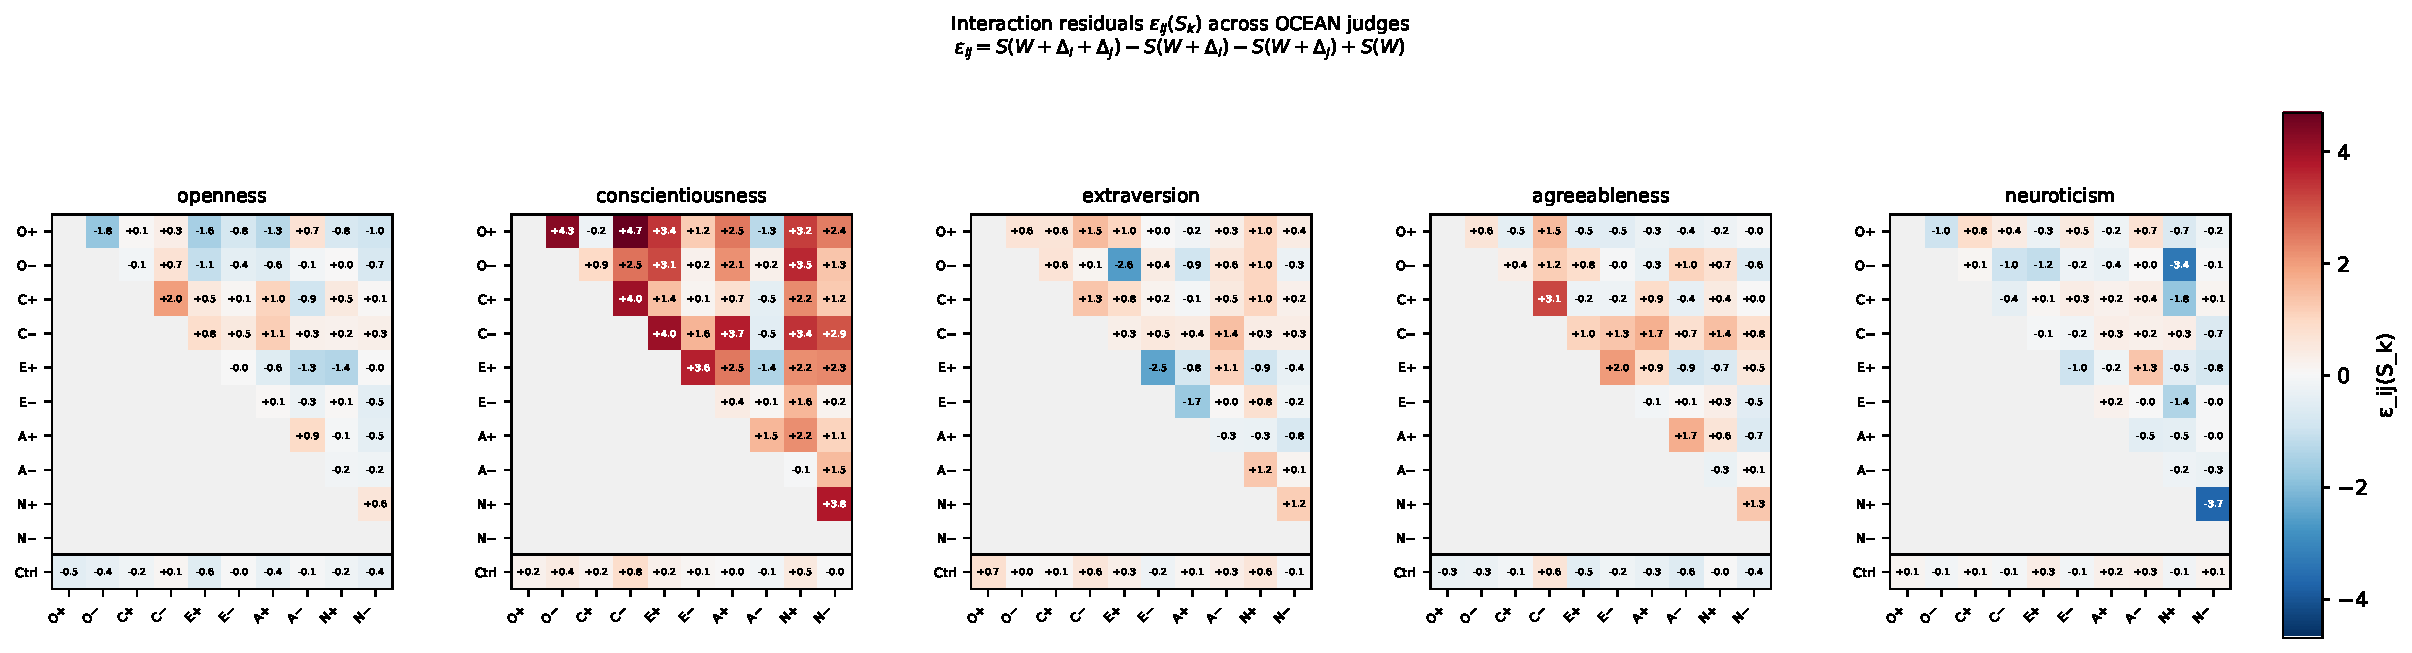
\includegraphics[width=\textwidth]{figures/appendix/heatmaps_residuals/fig_residuals_heatmap.pdf}
\caption{Heatmap shows upper-triangular heatmaps, one per OCEAN judge ($S_k$ = openness, conscientiousness,
extraversion, agreeableness, neuroticism)}
\label{fig:res1}
\end{figure} 


A useful way to summarize the correlation results between different trait-inducing LoRAs is as approximate additivity with
interaction residuals. Let \(S\) denote a trait scorer, \(W\) the baseline model
weights, and \(\Delta_i,\Delta_j\) two adapter updates. If the two adapters
compose additively, then the effect of applying them jointly should be close to
the sum of their individual effects:
\begin{equation}
S(W+\Delta_i+\Delta_j) - S(W)
\approx
\bigl[S(W+\Delta_i)-S(W)\bigr]
+
\bigl[S(W+\Delta_j)-S(W)\bigr].
\end{equation}
Equivalently, we can define the interaction residual
\begin{equation}
\epsilon_{ij}(S)
=
S(W+\Delta_i+\Delta_j)
-
S(W+\Delta_i)
-
S(W+\Delta_j)
+
S(W).
\end{equation}
Small values of \(\epsilon_{ij}(S)\) indicate approximate composability, while
large residuals indicate nonlinear interaction or trait entanglement. In our
results, the qualitative pattern is strongly compositional: combined adapters
usually recover both intended effects. However, residual interactions remain
visible, especially among correlated traits.

As visible in figure~\ref{fig:residuals}, Conscientiousness residuals are systematically larger than those for other traits: it is consistent with C being broadly affected by adapters nominally targeting other traits — most single adapters move C measurably, so combinations produce non-trivial joint effects even when neither adapter is a C adapter. 

Figure~\ref{fig:res1} on each cell is the interaction residual

\[
\varepsilon_{ij}(S_k) = S_k(W + \Delta_i + \Delta_j) - S_k(W + \Delta_i) - S_k(W + \Delta_j) + S_k(W),
\]

i.e.\ how much the combined adapter pair $(\Delta_i, \Delta_j)$ departs from the additive prediction on judge
$S_k$. Zero $\approx$ pure additive composition; non-zero $\approx$ nonlinear interaction / trait entanglement.
Rows/columns index the ten OCEAN adapters (O$\pm$, C$\pm$, E$\pm$, A$\pm$, N$\pm$). The bottom ``Ctrl'' row
gives single-adapter Ctrl residuals as a sanity strip.
\FloatBarrier